\scanpage{25}
\figure{\handwritten{%
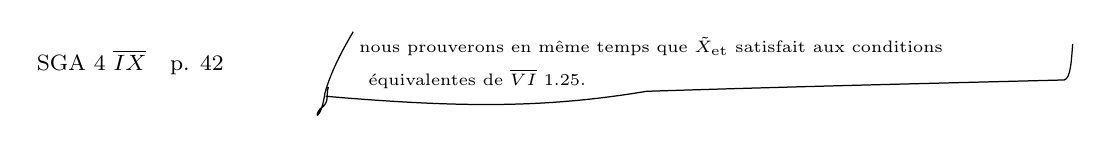
\begin{tikzpicture}[x=.009cm,y=-.009cm,font=\fontsize{8}{9}\selectfont]
\node[anchor=base west] at (160,83) {SGA 4 \(\overline{\text{\uline{IX}}}\)\quad p. 42};
\node[anchor=base west,font=\fontsize{6.5}{8}\selectfont] at (615,57) {nous prouverons en même temps que $\tilde{X}_{\mathrm{et}}$ satisfait aux conditions};
\node[anchor=base west,font=\fontsize{6.5}{8}\selectfont] at (628,104) {équivalentes de \(\overline{\text{\uline{VI}}}\) 1.25.};
\draw[line width=.45pt] (620,28) .. controls (601,60) and (587,89) .. (580,115)
 .. controls (575,151) and (563,151) .. (573,137)
 .. controls (588,128) and (581,117) .. (585,106);
\draw[line width=.45pt] (581,119) .. controls (779,136) and (895,135) .. (1034,112)
 .. controls (1254,105) and (1468,100) .. (1623,96)
 .. controls (1632,94) and (1633,70) .. (1635,45);
\end{tikzpicture}}}

\handwritten{(*) (Note pour la page 8.) Prouvons que la notion de constructibilité 2.3 pour un faisceau d'ensembles $F$ coïncide avec celle de \(\overline{\text{\uline{VI}}}\) 1.9.3. \deleted{Soit} La \deleted{en effet $C$ le \unsure{cas}}\inserted{question étant} locale sur $X$, on peut supposer $X$ affine \inserted{donc ``cohérent'', i.e.} quasi-compact et quasi-séparé. \deleted{Soit $C$ la catégorie \unsure{Soit $(C')$ le sous}\illegible{1}} \deleted{Je faut alors prouver que $F$ est constructible} Soit $C$ (resp. $C'$) la sous-catégorie \deleted{\unsure{pleine}}\inserted{strictement} pleine de $\tilde{X}_{\text{ét}}$ formée des $F$ constructibles au sens de 2.3, \deleted{\illegible{1}} \inserted{(resp. au sens de \(\overline{\text{\uline{VI}}}\) 1.9.3), il}}

% The opening conclusion shares the upper-left space of the cancellation graphic.
% The long paths, enclosing edges and nested cross-hatching below are source cancellation marks.
\reversemarginpar
\margin{\handwritten{%
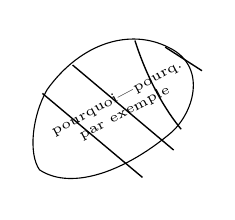
\begin{tikzpicture}[x=.012cm,y=-.012cm,font=\tiny]
\node[anchor=center,align=center,rotate=28] at (98,85) {\unsure{pourquoi|pourq.}\\par exemple};
\draw[line width=.4pt] (20,68) .. controls (56,18) and (108,3) .. (148,23)
 .. controls (189,42) and (177,90) .. (152,113)
 .. controls (105,153) and (47,176) .. (12,153)
 .. controls (0,136) and (4,96) .. (20,68);
\draw[line width=.5pt] (15,72)--(121,161);
\draw[line width=.5pt] (47,42)--(154,132);
\draw[line width=.5pt] (113,16) .. controls (127,60) and (147,92) .. (162,110);
\draw[line width=.5pt] (145,23)--(184,48);
\end{tikzpicture}}}
\normalmarginpar
\figure{\handwritten{%
\begin{tikzpicture}[x=.009cm,y=-.009cm,font=\fontsize{6.5}{8}\selectfont]
\node[anchor=base west,rotate=4] at (215,526) {faut prouver};
\node[anchor=base west,rotate=4] at (489,503) {que $C$ s'identifie à la catégorie des objets \uline{cohérents} de};
\node[anchor=base west,rotate=4] at (215,597) {\deleted{$\tilde{X}_{\mathrm{et}}$}};
\node[anchor=base west,rotate=4] at (329,579) {que $C=C'$;};
\draw[line width=.6pt] (490,495)--(1617,425);
\draw[line width=.5pt] (541,497)--(539,576)
 .. controls (521,607) and (526,584) .. (537,578)--(543,518);
\draw[line width=.6pt] (550,496)--(548,601)
 .. controls (533,632) and (537,602) .. (545,594)--(547,552);

\node[anchor=base west,rotate=4] at (574,558) {En vertu de \(\overline{\text{\uline{VII}}}\) 5.6 a),};
\node[anchor=base west,rotate=4] at (1153,515) {\deleted{l'objet final $X$ de} $\tilde{X}_{\mathrm{et}}$};
\node[anchor=base west,rotate=4] at (229,656) {\deleted{est cohérent, donc}};
\node[anchor=base west,rotate=4] at (585,622) {$C'$ est formé des objets \uline{cohérents} \deleted{\(\overline{\text{\uline{VI}}}\)} de $\tilde{X}_{\mathrm{et}}$ (2.5).};
\node[anchor=base west,rotate=4] at (230,708) {En vertu de \(\overline{\text{\uline{VI}}}\) 1.24, \deleted{\unsure{et}} et compte tenu du fait que $C$ est génératrice};
\node[anchor=base west,rotate=4] at (230,784) {dans $\tilde{X}_{\mathrm{et}}$ (2.7.2) et stable par limites inductives finies (2.\unsure{6|8} (i)),};
\node[anchor=base west,rotate=4] at (229,842) {il suffit de prouver que $C\subset C'$,};
\node[anchor=base west,rotate=4] at (941,757) {Mais il résulte de 2.7 que tout};
\node[anchor=base west,rotate=4] at (235,909) {$F\in\mathrm{ob}\,C$ est \uline{quasi-compact}, puisque un};
\node[anchor=base west,rotate=4] at (1065,823) {\deleted{$\unsure{G\in X_{\mathrm{et}}|G\in\mathrm{ob}\,X_{\mathrm{et}}}$ \unsure{représentable par un}}};
\node[anchor=base west,rotate=4] at (1155,784) {\inserted{$\unsure{G|C}\in\unsure{X_{\text{ét}}|X'_{\mathrm{et}}}$}};
\node[anchor=base west,rotate=4] at (231,983) {\deleted{schéma $X'\unsure{\in|C}$} qui est quasi-compact et quasi-séparé est quasi-compact};
\node[anchor=base west,rotate=4] at (229,1046) {comme objet de $\tilde{X}_{\mathrm{et}}$ \deleted{(5.6.1)} (\(\overline{\text{\uline{VII}}}\) 5.6.1).};

\node[anchor=base west,rotate=4] at (1151,952) {D'autre part pour};
\node[anchor=base west,rotate=4] at (233,1099) {\unsure{voir que} $\unsure{F|F'}\unsure{\in|\to}\unsure{\mathrm{ob}\,X'|X'}$ la diagonale};
\node[anchor=base west,rotate=4] at (1069,1020) {$\unsure{F\longrightarrow F\mathbin{\times}_{X}F|F\longrightarrow F\mathbin{\times}F}$ est quasi-compacte,};
\node[anchor=base west,rotate=4] at (231,1172) {il suffit de voir que \unsure{pour tout} \illegible{2}};
\node[anchor=base west,rotate=4] at (232,1238) {\unsure{et que}\illegible{2} \unsure{ce fait que $C$ est stable par produits}};
\node[anchor=base west,rotate=4] at (744,1156) {Comme $C$ est stable par};
\node[anchor=base west,rotate=4] at (1321,1097) {\deleted{limites projectives}};
\node[anchor=base west,rotate=4] at (1393,1062) {\inserted{produits}};
\node[anchor=base west,rotate=4] at (340,1248) {\inserted{(2.6 (ii))}};
\node[anchor=base west,rotate=4] at (243,1297) {finis, l'inclusion $C\subset C'$ est donc un cas particulier de 2.1.};

% Irregular enclosing edges and long oblique cancellation strokes.
\draw[line width=.6pt] (235,649)--(545,616);
\draw[line width=.5pt] (238,650)--(239,1219)--(252,1294)--(1598,1158)
 .. controls (1625,1157) and (1645,1112) .. (1650,1092);
\draw[line width=.5pt] (235,884)--(979,798)--(941,801)--(942,745)--(1591,697);
\draw[line width=.55pt] (239,646)--(586,1217);
\draw[line width=.55pt] (512,623)--(885,1222);
\draw[line width=.55pt] (624,480)--(1151,1198);
\draw[line width=.55pt] (917,472)--(1365,1170);
\draw[line width=.55pt] (1148,452)--(1602,1100);
\draw[line width=.55pt] (1418,452)--(1645,797);
\draw[line width=.45pt] (1556,429)--(1643,535);

% Nested cancelled attempt: right-hand band, lower-left band, and its tail.
\draw[line width=.6pt] (1156,929)--(1599,886)
 .. controls (1610,887) and (1610,922) .. (1618,943);
\draw[line width=.6pt] (1611,947)--(1610,1007)
 .. controls (1590,1029) and (1590,1006) .. (1608,1003);
\draw[line width=.55pt] (1610,1014)--(951,1086)--(952,1024)--(230,1075)--(222,1164)--(705,1110)--(704,1189)--(236,1233);
\draw[line width=.5pt] (228,1077)--(313,1147);
\draw[line width=.5pt] (244,1156)--(301,1069);
\draw[line width=.5pt] (289,1073)--(373,1140);
\draw[line width=.5pt] (316,1148)--(365,1060);
\draw[line width=.5pt] (359,1065)--(442,1130);
\draw[line width=.5pt] (386,1137)--(435,1053);
\draw[line width=.5pt] (430,1057)--(514,1122);
\draw[line width=.5pt] (459,1130)--(507,1047);
\draw[line width=.5pt] (501,1048)--(586,1113);
\draw[line width=.5pt] (532,1123)--(579,1039);
\draw[line width=.5pt] (572,1040)--(659,1105);
\draw[line width=.5pt] (605,1116)--(652,1032);
\draw[line width=.5pt] (645,1033)--(731,1097);
\draw[line width=.5pt] (678,1107)--(725,1023);
\draw[line width=.5pt] (718,1025)--(806,1089);
\draw[line width=.5pt] (751,1100)--(800,1016);
\draw[line width=.5pt] (793,1017)--(880,1081);
\draw[line width=.5pt] (824,1091)--(875,1009);
\draw[line width=.5pt] (868,1009)--(951,1073);
\draw[line width=.5pt] (897,1084)--(947,1001);
\draw[line width=.5pt] (1158,933)--(1251,989);
\draw[line width=.5pt] (1179,995)--(1241,924);
\draw[line width=.5pt] (1231,925)--(1336,977);
\draw[line width=.5pt] (1283,986)--(1330,914);
\draw[line width=.5pt] (1318,918)--(1420,969);
\draw[line width=.5pt] (1366,977)--(1418,906);
\draw[line width=.5pt] (1409,908)--(1506,958);
\draw[line width=.5pt] (1454,970)--(1499,899);
\draw[line width=.5pt] (1498,899)--(1599,946);
\draw[line width=.5pt] (1538,962)--(1584,903);
\draw[line width=.45pt] (258,1224)--(464,1139);
\draw[line width=.45pt] (402,1209)--(665,1119);
\end{tikzpicture}}}

\handwritten{En vertu de \(\overline{\text{\uline{VI}}}\) 2.9, b), il suffit de voir que $C$ est stable pour limites inductives finies et limites projectives finies, qu'elle est génératrice, et formée d'objets quasi-compacts. \deleted{\unsure{Et|et}} Compte tenu de 2.6 (i) et (2.7.2), il reste à prouver que tout $F\in\mathrm{ob}\,C$ est quasi-compact. Or 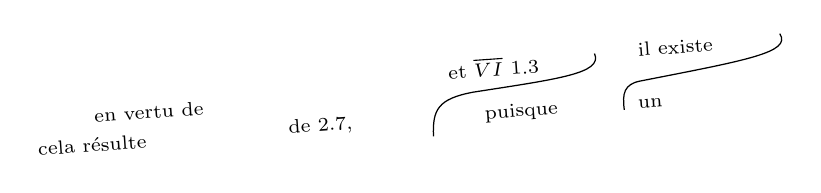
\begin{tikzpicture}[baseline=(correctionbase.base),x=.014cm,y=-.014cm,font=\scriptsize]
\node[anchor=base west,rotate=4] at (270,1578) {\deleted{cela résulte}};
\node[anchor=base west,rotate=4] at (321,1548) {\inserted{en vertu de}};
\node[anchor=base west,rotate=4] at (497,1558) {de 2.7,};
\node[anchor=base west,rotate=4] at (642,1509) {\deleted{et \(\overline{\text{\uline{VI}}}\) 1.3}};
\node[anchor=base west,rotate=4] at (675,1545) {\deleted{puisque}};
\node[anchor=base west,rotate=4] at (814,1488) {\inserted{il existe}};
\node[anchor=base west,rotate=4] (correctionbase) at (814,1535) {un};
\draw[line width=.45pt] (783,1485) .. controls (791,1503) and (750,1508) .. (673,1520)
 .. controls (641,1526) and (636,1536) .. (637,1560);
\draw[line width=.45pt] (951,1467) .. controls (962,1484) and (921,1491) .. (824,1510)
 .. controls (810,1513) and (808,1521) .. (810,1536);
\end{tikzpicture} $G\in\mathrm{ob}\,X_{\mathrm{et}}$ \deleted{\unsure{et}} qui est \inserted{un schéma} quasi-compact et quasi-séparé \deleted{\unsure{et} est} et un épimorphisme $G\longrightarrow F$. Or $G$ \deleted{\unsure{comme on}} est un objet quasi-compact de $\tilde{X}_{\mathrm{et}}$ (\(\overline{\text{\uline{VII}}}\) 5.6.1), donc $F$ est quasi-compact (\(\overline{\text{\uline{VI}}}\) 1.3), qfd.}

\handwritten{Bien entendu, il y aurait \inserted{eu} lieu de refondre les §§ 1,2 du présent exposé, \inserted{notamment} en les rattachant \deleted{\unsure{explicitement}} aux notions générales de \deleted{l'exposé} finitude de \(\overline{\text{\uline{VI}}}\). Nous laissons ce soin \deleted{\unsure{complémentaire}} de rédaction aux générations futures.}
% archive sheet number: 24
